\section{108 - K5 - AG 2.1, AG 4.1, FA 2.1, FA 2.2 - Zeitrad - MatKon}

\begin{langesbeispiel} \item[6] %PUNKTE DES BEISPIELS
Das Zeitrad ist die größte Sanduhr der Welt. Sie steht unweit des Heldenplatzes, am Rande des Stadtwäldchens in Ungarns Hauptstadt Budapest. Mit ihr feierte Ungarn am 1. Mai 2004 den Beitritt zur Europäischen Union.
		
\begin{center}
\resizebox{0.4\linewidth}{!}{\includegraphics{../_database/Bilder/108_sanduhr.eps}}\\
\begin{footnotesize}
Quelle: https://de.wikipedia.org/wiki/Zeitrad
\end{footnotesize}	
\end{center}

	
		
	Das Zeitrad ist ein Rad mit einem Durchmesser von 8 m, bei einer Breite von 2,5 m. Als Materialien wurden Edelstahl, Sicherheitsverbundglas und roter Granit verwendet. Das Gesamtgewicht der Uhr beträgt 60 Tonnen.
	
	Genau genommen handelt es sich bei der Uhr nicht um eine Sanduhr sondern um eine Glasgranulatuhr. Der Vorteil des Granulats gegenüber normalem Sand besteht darin, dass die gleich großen Körner die Oberfläche der Behälter nicht beschädigen und eine genau definierte Rieselgeschwindigkeit aufweisen.
	
	Die zwei Behälter, die die 4,5 Kubikmeter Glasgranulat beinhalten, wurden aus Verbundglas gefertigt. Etwa 0,0004932 m$^3$ Granulat rieseln pro Stunde vom oberen Behälter in den unteren.%Aufgabentext

\begin{aufgabenstellung}
\item %Aufgabentext

\ASubitem{Sei $S(t)$ die Menge des Glasgranulats im oberen Teil der Sanduhr und $t$ die Zeit in Stunden. Gib die Funktionsgleichung $S(t)$ an.} %Unterpunkt1
\Subitem{Berechne wie viele Tage vergehen müssen, bis das Glasgranulat zur Gänze im unteren Teil der Sanduhr liegt.} %Unterpunkt2

\item Bei den beiden Glasflächen handelt es sich um gleichschenklige Dreiecke. Der Zentriwinkel $\alpha$ hat eine Größe von $25,38^\circ$. 
	
	\begin{center}
	\resizebox{0.5\linewidth}{!}{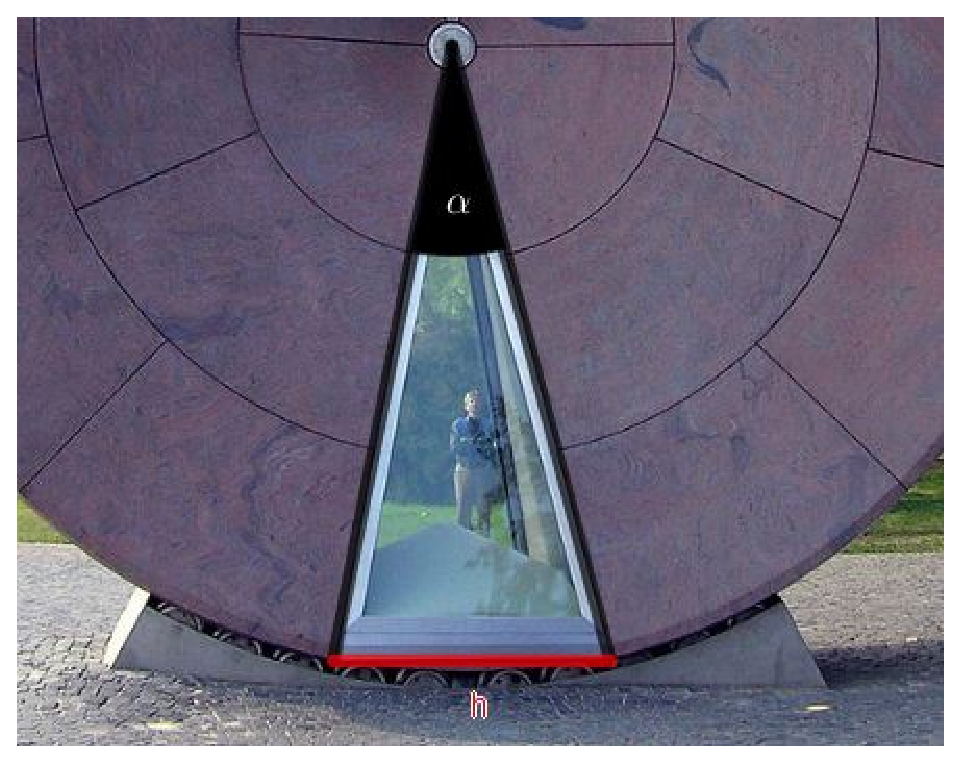
\includegraphics{../_database/Bilder/108_sanduhr2klein.eps}}
	\end{center}%Aufgabentext

\Subitem{Berechne die Länge der Basiskante (h) dieses Dreiecks.} %Unterpunkt1
\Subitem{Gib die Größe des Basiswinkel $\beta$ an.} %Unterpunkt2

\item Die Masse gibt an, wie leicht oder schwer und wie träge ein Körper ist. Die Masse eines Körpers ist im Unterschied zur Gewichtskraft an jedem beliebigen Ort gleich groß. Kennt man das Volumen $V$ des Körpers und die Dichte $\rho$ des Stoffes, aus dem er besteht, so kann man die Masse folgendermaßen berechnen:
	$$m=\rho\cdot V$$%Aufgabentext

\Subitem{Die Dichte von Glasgranulat liegt bei 2500\,kg/m$^3$, berechne die Masse der in der Sanduhr verwendeten Menge an Glasgranulat.} %Unterpunkt1
\Subitem{Kreuze die beiden richtigen Aussagen an!
	
	\multiplechoice[5]{  %Anzahl der Antwortmoeglichkeiten, Standard: 5
				L1={Die Masse ist indirekt proportional zum Volumen.},   %1. Antwortmoeglichkeit 
				L2={Die Dichte ist direkt proportional zur Masse.},   %2. Antwortmoeglichkeit
				L3={Der Graph der Masse in Abhängigkeit vom Volumen ergibt eine Parabel.},   %3. Antwortmoeglichkeit
				L4={Das Volumen ist immer doppelt so groß wie die Masse.},   %4. Antwortmoeglichkeit
				L5={Die Dichte ist indirekt proportional zum Volumen.},	 %5. Antwortmoeglichkeit
				L6={},	 %6. Antwortmoeglichkeit
				L7={},	 %7. Antwortmoeglichkeit
				L8={},	 %8. Antwortmoeglichkeit
				L9={},	 %9. Antwortmoeglichkeit
				%% LOESUNG: %%
				A1=2,  % 1. Antwort
				A2=5,	 % 2. Antwort
				A3=0,  % 3. Antwort
				A4=0,  % 4. Antwort
				A5=0,  % 5. Antwort
				}} %Unterpunkt2

\end{aufgabenstellung}

\begin{loesung}
\item \subsection{Lösungserwartung:} 

\Subitem{$S(t)=-0,0004932\cdot t+4,5$} %Lösung von Unterpunkt1
\Subitem{$S(t)=0 \Rightarrow t\approx 9124,0876$ Stunden also ungefähr 380 Tage} %%Lösung von Unterpunkt2

\setcounter{subitemcounter}{0}
\subsection{Lösungsschlüssel:}
 
\Subitem{Ein Punkt für die richtige Gleichung.} %Lösungschlüssel von Unterpunkt1
\Subitem{Ein Punkt für die richtige Anzahl der Tage.} %Lösungschlüssel von Unterpunkt2

\item \subsection{Lösungserwartung:} 

\Subitem{$\frac{h}{2}=4*\sin(12,69)\approx 0,879 \Rightarrow h=1,76$\,m} %Lösung von Unterpunkt1
\Subitem{$\beta=\dfrac{180-25,38}{2}=77,31^\circ$} %%Lösung von Unterpunkt2

\setcounter{subitemcounter}{0}
\subsection{Lösungsschlüssel:}
 
\Subitem{Ein Punkt für die richtige Länge der Basiskante.} %Lösungschlüssel von Unterpunkt1
\Subitem{Ein Punkt für den richtigen Basiswinkel.} %Lösungschlüssel von Unterpunkt2

\item \subsection{Lösungserwartung:} 

\Subitem{$V=4,5; \rho=2500 \Rightarrow m=11.250$\,kg} %Lösung von Unterpunkt1
\Subitem{MC: Lösungen siehe oben} %%Lösung von Unterpunkt2

\setcounter{subitemcounter}{0}
\subsection{Lösungsschlüssel:}
 
\Subitem{Ein Punkt für die richtige Masse.} %Lösungschlüssel von Unterpunkt1
\Subitem{Ein Punkt für die richtigen MC-Antworten.} %Lösungschlüssel von Unterpunkt2

\end{loesung}

\end{langesbeispiel}